\chapter{The Ising Magnet and the Liquid--Gas Transition}

You already know the phenomenon: water boils, liquid turns into vapor, and somewhere behind that familiar fact there is a phase transition. In this lecture Leonard Susskind takes a deliberately indirect route. Instead of beginning with van der Waals, he goes back to a system we have already studied, the Ising magnet, and shows that the same mathematics can be read as a model of the liquid--gas transition. These notes follow that order closely, using the transcript as the main guide and retaining a few blackboard frames where the lecture literally builds the argument on the board; the lecture record behind this chapter also reflects the curation work of LazyingArt LLC and Video2Book.

\section{From Boiling Water to the Ising Magnet}

The lecture begins with boiling water and immediately narrows the objective. We are not going to develop the liquid--gas transition in the standard van der Waals way, even though that approach is elegant and historically central. Instead, we will use the Ising magnet as a mathematically equivalent route.

That choice determines the whole rhythm of the lecture. Before any serious fluid language appears, we back up and reconstruct the Ising model: what the spin variables are, where the energy lives, what a broken bond costs, how a magnetic field enters, and why mean field is good enough to reveal the qualitative mechanism of a phase transition. Only after that machinery is in place do we reinterpret the same system as a lattice gas. The target is the liquid--gas transition, but the road to it runs through magnetism.

\section{Recap of Ising Energetics and Mean Field}

At each lattice site \(i\) we place a spin variable
\begin{equation}
\sigma_i=\pm 1.
\end{equation}
The Ising energy is not attached to a site by itself, but to links between neighboring sites. In the convention used in this lecture we write
\begin{equation}
E_{\text{Ising}}=-J\sum_{\langle ij\rangle}\sigma_i\sigma_j+h\sum_i \sigma_i.
\end{equation}
Here \(\langle ij\rangle\) denotes nearest-neighbor links, and \(J>0\) is the ferromagnetic coupling. If two neighboring spins are parallel, then \(\sigma_i\sigma_j=+1\) and the link energy is \(-J\). If they are anti-parallel, then \(\sigma_i\sigma_j=-1\) and the link energy is \(+J\). Therefore a broken bond costs
\begin{equation}
\Delta E_{\text{broken bond}}=(+J)-(-J)=2J.
\end{equation}

The all-aligned state is the ground state. If \(N\) is the number of sites of an infinite hypercubic lattice in \(d\) dimensions, then the number of links is \(dN\), so the ground-state energy is
\begin{equation}
E_{\text{ground}}=-J\,N_{\text{links}}=-J\,dN.
\end{equation}
The lecture insists on a simple but important point: this constant part of the energy is not what matters. We are free to shift the zero of energy. What matters is the difference between aligned and anti-aligned links, or between spin up and spin down in a field.

The site term \(h\sum_i \sigma_i\) acts independently on each spin. In the present convention, positive \(h\) lowers the energy when \(\sigma_i=-1\). Thus the link term wants neighboring spins to agree, while the field term, if present, favors one orientation over the other.

\begin{remark}
The blackboard discussion wanders through a few sign corrections. We will keep one convention throughout:
\[
E_{\text{field}}=h\sum_i \sigma_i.
\]
With this choice, positive \(h\) favors \(\sigma=-1\). The later reduced equation
\[
\frac{yT}{2dJ}=\tanh(y-\beta h)
\]
is then consistent with the visible board formula.
\end{remark}

Now we recall the mean-field idea. Mean field is not exact in one dimension; indeed it predicts a phase transition there when there is none. But in two dimensions and higher it becomes qualitatively useful, and by three dimensions it is already rather good. The reason is simple: the more neighbors a spin has, the more plausible it is to replace the actual surrounding spins by an average value.

\section{Self-Consistency for the Average Spin}

Take one spin \(\sigma\) and imagine it deep in the interior of a large sample. It has \(2d\) nearest neighbors. Mean field replaces those neighbors by their average value \(\bar{\sigma}\).

\begin{figure}[h]
\centering

\includegraphics[width=0.82\textwidth]{lecture_10_figure_02.png}
\caption{Mean-field self-consistency equation for \(\bar{\sigma}\) as it appears on the board. The right edge is cropped, but the one-spin coefficient \(-2dJ\bar{\sigma}+h\) and the self-consistency structure are visible.}
\end{figure}

\begin{figure}[h]
\centering
\begin{tikzpicture}[scale=1.15]
\fill (0,0) circle (2.4pt);
\node[below] at (0,-0.1) {$\sigma$};

\node at (1.6,0) {$\times$};
\node at (-1.6,0) {$\times$};
\node at (0,1.35) {$\times$};
\node at (0,-1.35) {$\times$};

\draw (0.18,0) -- (1.15,0);
\draw (-0.18,0) -- (-1.15,0);
\draw (0,0.18) -- (0,0.95);
\draw (0,-0.18) -- (0,-0.95);

\node[right] at (1.95,0.28) {$\bar{\sigma}$};
\node[left] at (-1.95,0.28) {$\bar{\sigma}$};
\node[above] at (0,1.62) {$\bar{\sigma}$};
\node[below] at (0,-1.62) {$\bar{\sigma}$};
\end{tikzpicture}
\caption{The mean-field picture used in the lecture: one central spin interacting with \(2d\) neighbors, each replaced by the same average value \(\bar{\sigma}\).}
\end{figure}

With that approximation, the energy of the chosen spin becomes
\begin{equation}
E_{\text{mf}}(\sigma)=(-2dJ\,\bar{\sigma}+h)\sigma.
\end{equation}
At this point the many-body problem has been reduced to a one-spin statistical mechanics problem with a parameter \(\bar{\sigma}\) that is not yet known.

The one-spin partition function is
\begin{align}
Z_1
&=\sum_{\sigma=\pm 1} e^{-\beta E_{\text{mf}}(\sigma)} \\
&=\sum_{\sigma=\pm 1} e^{-\beta(-2dJ\bar{\sigma}+h)\sigma} \\
&=2\cosh\!\big[\beta(2dJ\bar{\sigma}-h)\big].
\end{align}
The thermal average of the chosen spin is therefore
\begin{align}
\langle \sigma\rangle
&=\frac{1}{Z_1}\sum_{\sigma=\pm 1}\sigma\,e^{-\beta E_{\text{mf}}(\sigma)} \\
&=\tanh\!\big[\beta(2dJ\bar{\sigma}-h)\big].
\end{align}
Mean field now makes its decisive move: the average spin of the chosen site is assumed to equal the average of its neighbors. That is the self-consistency condition,
\begin{equation}
\bar{\sigma}=\tanh\!\big[\beta(2dJ\bar{\sigma}-h)\big].
\end{equation}

The lecture then introduces a reduced variable
\begin{equation}
y=2dJ\,\beta\,\bar{\sigma},
\end{equation}
so that \(\bar{\sigma}=yT/(2dJ)\). The self-consistency equation becomes
\begin{equation}
\frac{yT}{2dJ}=\tanh(y-\beta h).
\end{equation}
This is the right form for the next step, because it turns the problem into the intersection of a straight line and a fixed nonlinear curve.

\section{Graphical Solution and the Critical Temperature}

The lecture now clears away the clutter and asks first what happens when the field is turned off:
\begin{equation}
\frac{yT}{2dJ}=\tanh y.
\end{equation}
The left-hand side is a straight line through the origin with slope \(T/(2dJ)\). The right-hand side is the hyperbolic tangent.

\begin{figure}[h]
\centering

\includegraphics[width=0.78\textwidth]{lecture_10_figure_03.png}
\caption{The reduced scalar equation, rewritten just before the graphical analysis begins.}
\end{figure}

\begin{figure}[h]
\centering
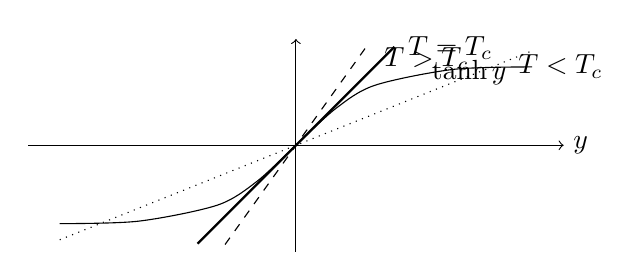
\begin{tikzpicture}[scale=1.0]
\draw[->] (-3.4,0) -- (3.4,0) node[right] {$y$};
\draw[->] (0,-1.35) -- (0,1.35);

\draw[smooth] plot coordinates {
(-3,-0.995) (-2,-0.964) (-1,-0.761) (-0.5,-0.462) (0,0)
(0.5,0.462) (1,0.761) (2,0.964) (3,0.995)};
\node at (2.2,0.92) {$\tanh y$};

\draw[dashed] (-0.9,-1.26) -- (0.9,1.26);
\node[right] at (1.0,1.1) {$T>T_c$};

\draw[thick] (-1.25,-1.25) -- (1.25,1.25);
\node[right] at (1.3,1.23) {$T=T_c$};

\draw[dotted] (-3.0,-1.2) -- (3.0,1.2);
\node[right] at (2.7,1.0) {$T<T_c$};
\end{tikzpicture}
\caption{The graphical solution of \(\frac{yT}{2dJ}=\tanh y\). At high temperature the line is steep and intersects only at the origin. At the critical temperature it is tangent at the origin. Below criticality it intersects at two additional nonzero points.}
\end{figure}

At high temperature the slope \(T/(2dJ)\) is large, so the line is steep and the only intersection is at the origin. Therefore \(y=0\), and since \(y\propto \bar{\sigma}\), there is no magnetization.

As we lower the temperature, the slope decreases. At the critical point the line becomes tangent to \(\tanh y\) at the origin. Since
\begin{equation}
\left.\frac{d}{dy}\tanh y\right|_{y=0}=1,
\end{equation}
the tangency condition is simply
\begin{equation}
\frac{T_c}{2dJ}=1.
\end{equation}
Thus the mean-field critical temperature is
\begin{equation}
T_c=2dJ.
\end{equation}

Below that temperature the line is shallower still, and two nonzero intersections appear, one with \(y>0\) and one with \(y<0\). That is the onset of spontaneous magnetization. The system has developed two symmetry-related solutions.

This value of \(T_c\) is not exact; it is a mean-field estimate. The lecture emphasizes that it becomes exact only in large dimension. For \(d=2\) it is noticeably off, and for \(d=3\) it is already fairly good. But the important point is that mean field captures the qualitative structure correctly.

The magnetic name for \(T_c\) is the Curie temperature. In the broader language of phase transitions it is simply the critical temperature.

\section{Question \& Answer: What Jumps, and What Does Not?}

Once the two nonzero branches appear, the lecture slows down, because the mathematics has produced an ambiguity. If \(h=0\) exactly and \(T<T_c\), the mean-field equation has two symmetry-related nonzero solutions. Which one does the system choose?

The answer is that an arbitrarily small field breaks the symmetry and selects one branch. In a macroscopic sample there is always some tiny bias somewhere, so the exact \(h=0\) idealization is a knife-edge limit.

\begin{figure}[h]
\centering
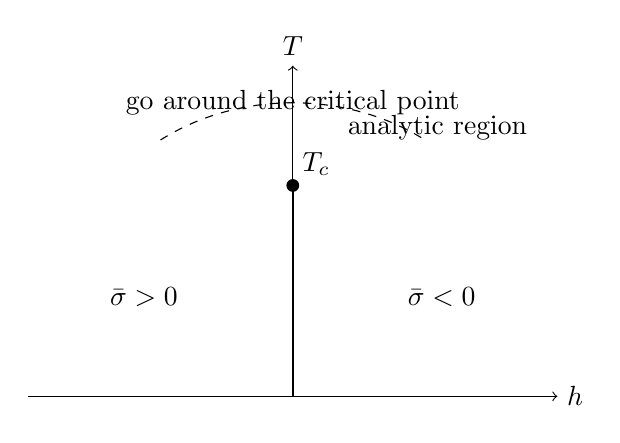
\begin{tikzpicture}[scale=1.05]
\draw[->] (-3.2,0) -- (3.2,0) node[right] {$h$};
\draw[->] (0,0) -- (0,4.0) node[above] {$T$};

\draw[thick] (0,0) -- (0,2.55);
\fill (0,2.55) circle (2.2pt);
\node[above right] at (0,2.55) {$T_c$};

\node at (-1.8,1.2) {$\bar{\sigma}>0$};
\node at (1.8,1.2) {$\bar{\sigma}<0$};
\node at (1.75,3.25) {analytic region};

\draw[dashed] (-1.6,3.1) .. controls (-0.65,3.7) and (0.65,3.7) .. (1.6,3.1);
\node at (0,3.55) {go around the critical point};
\end{tikzpicture}
\caption{Mean-field \(T\)-\(h\) plane in the convention \(E_{\text{field}}=h\sum_i \sigma_i\). Below \(T_c\), the line \(h=0\) is the place where the two symmetry-related branches meet. Going around the critical point avoids the jump.}
\end{figure}

\subsection{Question \& Answer}

\paragraph{Question.} What exactly jumps? Does the magnetization go continuously to zero, or does it jump discontinuously?

\paragraph{Answer.} Both statements are true, but in different directions in parameter space. At the critical point itself the magnetization tends to zero continuously from every direction:
\begin{equation}
\lim_{(T,h)\to(T_c,0)} \bar{\sigma}(T,h)=0.
\end{equation}
If we move along the coexistence line \(h=0\) with \(T<T_c\), the two branches remain distinct:
\begin{equation}
\bar{\sigma}(T,0^\pm)=\pm m_0(T), \qquad m_0(T)>0,\qquad T<T_c.
\end{equation}
So the critical point is a continuous endpoint, but below it the passage from one branch to the other is discontinuous.

\paragraph{Question.} What happens on the line itself?

\paragraph{Answer.} In the idealized symmetric problem, the system ``does not know what to do.'' The two branches are equally available. In any real experiment a tiny residual field, or some other microscopic bias, chooses one of them.

\paragraph{Question.} Can one go from negative magnetization to positive magnetization without a sharp jump?

\paragraph{Answer.} Yes. If one insists on staying at fixed \(T<T_c\) and varying only the field, there is a jump at \(h=0\). But if one is allowed to move in the full \((T,h)\)-plane, one can go around the critical point. Then the change from one sign of magnetization to the other is smooth. This is one of the lecture's central conceptual points: locally there is a discontinuity, globally there is still a continuous path around it.

The lecture does not pause here to sort the formal taxonomy of first-order and second-order transitions in full detail. What matters for the present purpose is the geometry: below the critical point there is a discontinuous flip across the coexistence line, while the critical point itself is where the order parameter dies continuously.

\section{Chemical Potential and the Box Picture}

Only after this magnetic story is in hand does the lecture pivot to fluids. We imagine a box whose interior is at lower potential energy than the exterior. Particles can pass through the walls, so the number of particles inside is not fixed. The one-particle energy difference between inside and outside is called the chemical potential \(\mu\).

\begin{figure}[h]
\centering
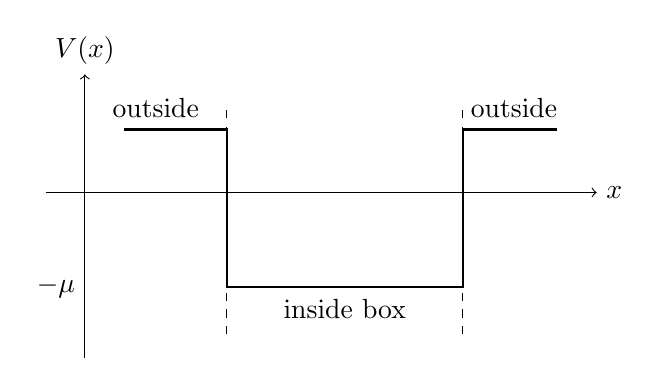
\begin{tikzpicture}[scale=1.0]
\draw[->] (-0.5,0) -- (6.5,0) node[right] {$x$};
\draw[->] (0,-2.1) -- (0,1.5) node[above] {$V(x)$};

\draw[thick] (0.5,0.8) -- (1.8,0.8) -- (1.8,-1.2) -- (4.8,-1.2) -- (4.8,0.8) -- (6.0,0.8);
\draw[dashed] (1.8,-1.8) -- (1.8,1.1);
\draw[dashed] (4.8,-1.8) -- (4.8,1.1);

\node at (0.9,1.08) {outside};
\node at (5.45,1.08) {outside};
\node at (3.3,-1.48) {inside box};
\node[left] at (0,-1.2) {$-\mu$};
\end{tikzpicture}
\caption{The box picture from the lecture. Inside the box the one-particle energy is lower. The walls are permeable, so the particle number inside is allowed to fluctuate.}
\end{figure}

Because lower energy is favored by the Boltzmann factor, particles prefer to sit inside the box. The stronger the chemical potential, the greater the equilibrium density inside. The point of this picture is not chemistry in any detailed sense; it is only to isolate a control parameter that tunes density.

In this setting the relevant partition function is grand canonical:
\begin{equation}
Z=\sum_N \sum_{\text{conf}_N} e^{-\beta E+\beta \mu N}.
\end{equation}
The lecture does not perform this sum. It only uses the formula to make the role of \(\mu\) explicit. The number of particles fluctuates, and the chemical potential is the parameter that controls the average density.

Now comes the fluid-language description of the transition. Hold the temperature fixed and vary \(\mu\). Then the density is some function of \(\mu\). At a liquid--gas transition, that function ceases to vary smoothly and instead jumps: the density changes discontinuously from a low-density gas to a high-density liquid.

\begin{remark}
The lecture deliberately stops short of a pressure calculation. Pressure could be introduced as a function of temperature and chemical potential, and one could then describe boiling at fixed pressure, but that computation is not carried out here and should not be invented on its behalf.
\end{remark}

\subsection{Question \& Answer}

\paragraph{Question.} How does one vary the chemical potential in practice?

\paragraph{Answer.} In the lecture the cleanest thought experiment is to lower the one-particle potential energy inside the box and thereby ``pull'' particles in. In practice, for an ordinary fluid, one usually varies the pressure. Pressure is the more natural experimental control, and the point at which boiling occurs depends on it. The thought experiment with \(\mu\) is used because it makes the logic of the density jump transparent.

\section{The Lattice Gas Hidden Inside the Ising Model}

We now return to the Ising system and read it in a new language. Let \(\sigma=-1\) mean that a lattice site is empty, and \(\sigma=+1\) mean that it is occupied by one particle. Then the all-down magnetic ground state becomes empty space.

\begin{figure}[h]
\centering

\includegraphics[width=0.74\textwidth]{lecture_10_figure_04.png}
\caption{The moment where the lattice-gas interpretation is introduced on the board: \(\sigma=-1\) means an empty site.}
\end{figure}

The occupancy dictionary is
\begin{equation}
\sigma_i=-1 \Longleftrightarrow n_i=0,
\qquad
\sigma_i=+1 \Longleftrightarrow n_i=1.
\end{equation}

\begin{figure}[h]
\centering
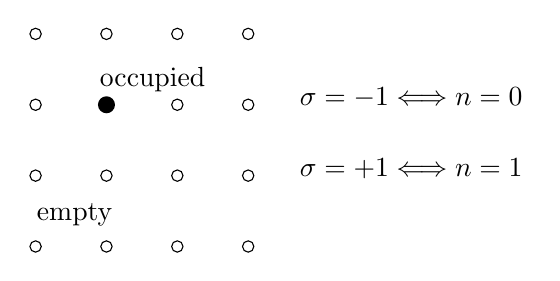
\begin{tikzpicture}[scale=0.9]
\foreach \x in {0,1,2,3}
  \foreach \y in {0,1,2,3}
    \draw (\x,\y) circle (0.08);

\fill (1,2) circle (0.12);

\node at (5.3,2.1) {$\sigma=-1 \Longleftrightarrow n=0$};
\node at (5.3,1.1) {$\sigma=+1 \Longleftrightarrow n=1$};
\node at (1.65,2.35) {occupied};
\node at (0.55,0.45) {empty};
\end{tikzpicture}
\caption{A clean lattice-gas reading of the two spin values. Since \(\sigma\) can only be \(\pm 1\), double occupancy is automatically forbidden.}
\end{figure}

This already gives the first ingredient of a liquid--gas model: hard-core repulsion. The Ising variable does not allow \(\sigma=2\), so it does not allow two particles on the same site. Occupancy is either \(0\) or \(1\), never more. That is an infinite on-site repulsion built in from the start.

The second ingredient is attraction. For that we return to the link energy and count explicitly. The lecture does this in two dimensions, where the bookkeeping is easy to see. We subtract the constant energy of the empty lattice and declare that state to have zero energy.

\begin{figure}[h]
\centering

\includegraphics[width=0.78\textwidth]{lecture_10_figure_05.png}
\caption{Energy counting for one particle, two separated particles, and two close particles. The numerical comparison is the essential new content.}
\end{figure}

One occupied site is one flipped spin. In two dimensions it breaks four bonds, and each broken bond costs \(2J\). Therefore
\begin{align}
E_{1\text{ particle}} &= 4(2J)=8J, \\
E_{2\text{ particles, far apart}} &= 2\cdot 8J = 16J.
\end{align}
If the two particles are nearest neighbors, the bond between them is no longer broken. The total number of broken bonds is then six rather than eight, so
\begin{equation}
E_{2\text{ particles, nearest neighbors}}=6(2J)=12J.
\end{equation}
The effective nearest-neighbor interaction is therefore attractive:
\begin{equation}
12J-16J=-4J.
\end{equation}

\begin{figure}[h]
\centering
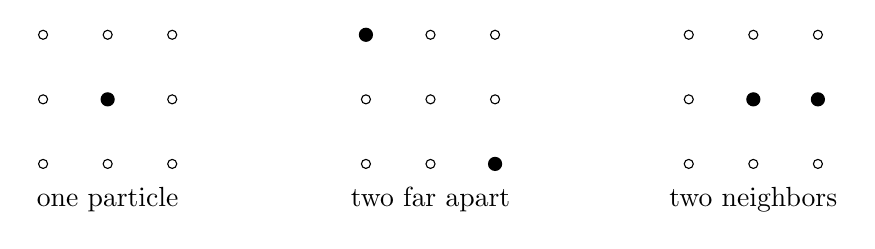
\begin{tikzpicture}[scale=0.82]
\foreach \x in {0,1,2}
  \foreach \y in {0,1,2}
    \draw (\x,\y) circle (0.07);
\fill (1,1) circle (0.11);
\node at (1,-0.55) {one particle};

\begin{scope}[xshift=5.0cm]
\foreach \x in {0,1,2}
  \foreach \y in {0,1,2}
    \draw (\x,\y) circle (0.07);
\fill (0,2) circle (0.11);
\fill (2,0) circle (0.11);
\node at (1,-0.55) {two far apart};
\end{scope}

\begin{scope}[xshift=10.0cm]
\foreach \x in {0,1,2}
  \foreach \y in {0,1,2}
    \draw (\x,\y) circle (0.07);
\fill (1,1) circle (0.11);
\fill (2,1) circle (0.11);
\node at (1,-0.55) {two neighbors};
\end{scope}
\end{tikzpicture}
\caption{The three lattice configurations whose bond counting gives \(8J\), \(16J\), and \(12J\) in two dimensions.}
\end{figure}

This is exactly the structure needed for a liquid--gas transition: an infinite short-range repulsion at zero separation, and a modest attraction at one lattice spacing. The attraction is not overwhelming; it is just enough to make neighboring occupation energetically favorable.

What about the chemical potential? The field term provides it. When a site changes from empty to occupied, \(\sigma\) changes from \(-1\) to \(+1\), so the field contribution changes by
\begin{equation}
\Delta E_h = 2h.
\end{equation}
Thus the field changes the one-particle energy by a tunable amount, independently of \(J\). Up to an additive offset coming from the isolated-particle cost \(8J\), it plays the role of a chemical potential control. In the present sign convention, increasing \(h\) disfavors occupied sites; equivalently, the effective chemical tendency to occupy a site grows when \(h\) is lowered.

\begin{remark}
The lecture only needs the structural statement: \(J\) fixes the interaction between neighboring particles, while \(h\) controls the one-body occupancy cost. The exact identification of \(h\) with the thermodynamic chemical potential is therefore understood only up to sign convention and an additive constant.
\end{remark}

The density is obtained directly from the spin variable:
\begin{equation}
n_i=\frac{1+\sigma_i}{2},
\qquad
\rho=\langle n_i\rangle=\frac{1+\bar{\sigma}}{2}.
\end{equation}
Since \(\bar{\sigma}\in[-1,1]\), the density lies in the expected range \(\rho\in[0,1]\).

Now the phase diagram translates immediately. Above the critical temperature, the magnetization changes smoothly when the field is varied, so the density also changes smoothly when the chemical potential is varied. Below the critical temperature, the magnetization jumps across the coexistence line, so the density jumps from low to high. In that language, the magnetic phase transition has become the liquid--gas transition.

This is the lecture's final payoff. The Ising magnet is not merely analogous to the liquid--gas system; it is the same mathematics in a different physical costume. The two descriptions even share the same universality class. Near the critical point the interesting quantities behave with nontrivial critical exponents, and the lecture closes by emphasizing that the magnetic and liquid--gas transitions fall into the same class of critical behavior, even though the microscopic stories look different.

\section{Summary}

The lecture began with boiling water and reached it by a detour through magnetism. First we reconstructed the Ising model: link energy, broken-bond cost, the field term, and the mean-field reduction to one spin in an average environment. That gave the self-consistency equation
\[
\bar{\sigma}=\tanh\!\big[\beta(2dJ\bar{\sigma}-h)\big],
\]
and, after the introduction of \(y=2dJ\beta\bar{\sigma}\), the graphical equation
\[
\frac{yT}{2dJ}=\tanh(y-\beta h).
\]
From that graph we read off the mean-field critical temperature \(T_c=2dJ\), the two symmetry-related magnetized branches below \(T_c\), and the distinction between continuity at the critical point and the jump across the coexistence line.

Then we changed language without changing mathematics. Empty and occupied lattice sites were identified with \(\sigma=-1\) and \(\sigma=+1\). Hard-core repulsion was automatic, and explicit bond counting revealed a short-range attraction of strength \(4J\) in two dimensions. Finally,
\[
\rho=\frac{1+\bar{\sigma}}{2}
\]
translated magnetization into density. The jump of \(\bar{\sigma}\) became the jump from vapor to liquid, and the Ising magnet became a model of boiling.